\documentclass[12pt]{article}
\usepackage[utf8]{inputenc}
\usepackage{graphicx}
\usepackage{listings}
\usepackage{hyperref}
\usepackage{xcolor}
\usepackage{enumitem}
\usepackage{circuitikz}
\usepackage{tikz}
\usetikzlibrary{shapes.geometric, arrows}
\graphicspath{ {./images/} }
\tikzstyle{year} = [rectangle, rounded corners, minimum width=3cm, minimum height=1cm,text centered, draw=black, fill=orange!30]
\tikzstyle{arrow} = [thick,->,>=stealth]

\definecolor{codegreen}{rgb}{0,0.6,0}
\definecolor{codegray}{rgb}{0.5,0.5,0.5}
\definecolor{codepurple}{rgb}{0.58,0,0.82}
\definecolor{backcolour}{rgb}{0.95,0.95,0.92}

\lstdefinestyle{mystyle}{
    backgroundcolor=\color{backcolour},   
    commentstyle=\color{codegreen},
    keywordstyle=\color{magenta},
    numberstyle=\tiny\color{codegray},
    stringstyle=\color{codepurple},
  basicstyle=\ttfamily\footnotesize,
  breakatwhitespace=false,         
  breaklines=true,                 
  captionpos=b,                    
  keepspaces=true,                 
  numbers=left,                    
  numbersep=5pt,                  
  showspaces=false,                
  showstringspaces=false,
  showtabs=false,                  
  tabsize=2
}

\lstset{style=mystyle}

\title{TigerTown Semiconductor
\begin{center}
    \emph{Report to Director on Gen II MOSFETs}
    \centerline{\includegraphics[width=12cm] {TigerTown Logo.PNG}}
\end{center}
}


\author{Daniel Simone}
\date{19 November 2021}

\begin{document}

\maketitle
\pagebreak

\section{Project Administrative Information}
\subsection{R\&D Division}
Sub-Division: ECE 308 \\ Laboratory Section: B01 \\ Director of R\&D: James Sturm
\subsection{Table of Contents}
\tableofcontents
\pagebreak

\section{Engineering Goals}
The three main engineering goals for an inverter gate include the power, speed, and cost of the device. The theoretical power, speed, and costs can be calculated before the device performance. However, to calculate these parameters, an understanding of the dimensions of the inverter is necessary.

\subsection{Inverter Dimensions}
\subsubsection{Length}
The total length of the CMOS inverter can be considered 200 microns, including 75 per nMOS and pMOS transistors, and 50 for three spaces before, between, and after the CMOS (the space after the CMOS is part of the space before the next CMOS, so it only has to be counted once).
This is demonstrated in figure 2.1.1:
\\\centerline{\includegraphics[width=18cm] {Inverter Size Diagram.PNG}}
\begin{center}
\\\emph{Figure 2.1.1: Inverter Length Diagram}
\end{center}

\subsubsection{Width}
The width of the nMOS MOSFET can be considered as 25 microns. However, since the mobility of a pMOS channel tends to be half that of an nMOS channel, in order to keep the device transconductance the same for the pMOS, the width of the pMOS can be considered as 50 microns, making the device's total width 50 microns. An additional 25 microns is required to pad one side of the inverter, so it does not contact the next inverter. The other side is padded by the next inverter's 25 microns padding. This is seen from a calculation of the device transconductance factor:
\\
\\\[K_P = Ratio_{mobility} \times Ratio_{area} \times K_N\]
\[K_P = \frac{1}{2} \times 2 \times K_N\]
\[K_P = K_N\]
\subsubsection{Channel and Inverter Area}
This provides for a total area per nMOS channel of:
\\
\\\centerline{\emph{625 microns squared}}
\\
\\And a total area per pMOS channel of:
\\
\\\centerline{\emph{1250 microns squared}}
\\
\\And a total area of the inverter of:
\\
\\\centerline{\emph{15000 microns squared}}

\subsection{Power}
The power consumption of the CMOS inverter can be calculated by modelling the inverter as a resistor, nMOS FET, and capacitor. The inverter would be modeled as follows:
\\
\begin{center}
\begin{circuitikz} 
\draw (0, 0) to[R, o-o] (0, -2)
  node[nmos, anchor=D]]{};
\draw (0, -3.5) node[ground]{};
\draw (0, -2) to[C] (2, -2);
\draw (2, -2) -- (2, -3.5);
\draw (2, -3.5) node[ground]{};
\end{circuitikz}
\\\emph{Figure 2.2.1: CMOS Inverter Model}
\end{center}
Then, using the source voltage, the resistance of the top FET, represented as a resistor, and the capacitance of the gate the CMOS is connected to, represented as a capacitor, power loss can be calculated.

\subsubsection{Power Loss from Resistance}
First, to calculate the power loss from resistance, we can use the following formula, which calculates the power loss from the resistance of a P-type transistor:
\[P_R = \frac{V_{DD}^2}{2R_P} \]
This requires calculating the resistance, which can be calculated using the following formula:
\[R = \frac{L_{channel}}{W_{channel} \times H \times \mu \times N_D \times q} \]
Given the following parameters,
\[L_P = 25um \]
\[W_P = 50um \]
\[H = 0.5um \]
\[\mu _P = 450\frac{cm^2}{Vs}* \]
\[N_D = 10^{17} cm^{-3}\]
\[q = 1.60217662 × 10^{-19}C \]
\emph{*Note that the value from mobility was taken from the following mobility vs. doping curve, where the red line represents electron mobility, and blue line represents hole mobility:}
\\
\\\centerline{\includegraphics[width=12cm] {Mobility.PNG}}
\begin{center}
\\\emph{Figure 2.2.1.1: Mobility vs. Doping Curve}
\end{center}
\\
\\It is possible to calculate the resistance of both types of transistors:
\[R_P = 891742465 \Omega\]
Then, given a default voltage,
\[V_{DD} = 10V \]
This makes it possible to calculate average power loss to resistance per inverter:
\[P_R = \frac{10V^2}{2 \times 891742465 \Omega} \]
\[P_R = 0.00000005607W \]
\[P_R \approx 56nW \]
\subsubsection{Power Loss from Capacitance}
\\Second, to calculate the power loss from capacitance, we can use the following formula, which measures power lost to the capacitor in the next transistor, to which the current CMOS's output line is connected:
\[P_C = f_{sw} \times \frac{1}{2} \times C_{out} \times V_{DD}^2 \]
This requires calculating the capacitance of the pMOS and nMOS gates and then averaging them, assuming that the output capacitor has an equally likely change of being a pMOS or nMOS gate, which can be calculated using the following formula:
\[C = \frac{W \times L \times \epsilon _{SiO2}}{H} \]
Given the following parameters,
\[L_N = 25um \]
\[L_P = 25um \]
\[W_N = 25um \]
\[W_P = 50um \]
\[H = 0.09um \]
\[\epsilon _{SiO2} = 3.0 \times 8.85418782 \times 10^{-12} m^{-3} kg^{-1} s^4 A^2\]
It is possible to calculate the capacitance of both types of transistors:
\[C_P = 2.3979583\times10^{-13}F\]
\[C_N = 1.1989792\times10^{-13}F\]
\[C_{avg} = 1.7984688\times10^{-13}F\]
Then, given a default voltage and frequency,
\[V_{DD} = 10V \]
\[F = 1MHz \]
This makes it possible to calculate average power loss to capacitance per inverter:
\[P_C = 1000000Hz \times \frac{1}{2} \times 1.7984688\times10^{-13}F \times 10V^2 \]
\[P_C = 0.000008992344W \]
\[P_C \approx 8992nW \]

\subsubsection{Total Power Loss}
Adding the two power calculations together, the power usage of one inverter can be calculated as:
\[P \approx 9048nW \approx 9uW \]


\subsection{Speed}
The speed of the MOSFET, assuming that it is symmetric (in this case, it was designed to be symmetric) and driving a gate similar to itself, can be calculated using the following formula:
\[\tau _{HL} = \tau _{LH} = \frac{5 \times L_N^2}{\mu _N \times V_{DD}} \]
Given the following parameters,
\[L_N = 25um \]
\[\mu _N = 700\frac{cm^2}{Vs} \]
\[V_{DD} = 10V \]
It is possible to calculate the delay of the CMOS inverter:
\[\tau _{HL} = \tau _{LH} = \frac{5 \times 25um^2}{700\frac{cm^2}{Vs} \times 10V} \]
\[\tau _{HL} = \tau _{LH} = 0.000000004464s \]
\[\tau _{HL} = \tau _{LH} \approx 4.5ns \]

\subsection{Cost}
Given that a 100mm wafer costs 500 dollars, the cost per inverter can be found by determining how many inverters fit on a wafer and dividing the wafer cost by the number of inverters.
\\
\\This can be accomplished with a python script, which counts the number of inverters that fit per strip of the wafer, as demonstrated by the simplified model in figure 2.4.1:
\\
\\\centerline{\includegraphics[width=8cm] {Python Code Model.PNG}}
\begin{center}
\\\emph{Figure 2.4.1: Python Code Model}
\end{center}
\\
\\The code implementing this model is as follows:
\begin{lstlisting}[language=Python, caption=Cost Per Inverter Code]
import math

R = 50000
total_cost = 500
D = 2 * R
total_height = R
running_height = 0
inverter_length = 200
inverter_width = 75
total_inverters = 0

# Calculate how many complete inverters fit along the diameter
total_inverters += D // inverter_length - 1
# Subtract 1 since one inverter would be cut off on the edge
running_height += inverter_width/2

# Get the initial theta and length across the circular disk
theta = 2 * (math.acos(running_height / R))
length_across = 2 * R * math.sin(0.5 * theta)

# Calculate the rest of the inverters on top and bottom of the diameter
while(True):
    total_inverters += 2 * (length_across // inverter_length)
    running_height += inverter_width
    if(total_height < running_height): break
    theta = 2 * (math.acos(running_height / R))
    length_across = 2 * R * math.sin(0.5 * theta)

print("The total number of inverters is: " + str(total_inverters))
print("The cost per inverter is: " + str(round((500 / total_inverters), 10)))

#Output:
#The total number of inverters is: 523397.0
#The cost per inverter is: 0.0009552978
\end{lstlisting}
\\
\\As is visible, the code finds that 523397 inverters fit on the wafer. This is less than the method of dividing the area of the wafer by the area of one inverter:
\[ N_{inverters} = \frac{Area_{wafer}}{Area_{inverter}} \approx \frac{7853.982mm^2}{0.015mm^2} \approx 523598 \]
Still, it is very close, suggesting that the spatial organization used in the script is close to the optimal configuration for spatially distributing the inverters.
\\
\\Thus, each inverter costs \$0.0009552978. More informatively, 1,000,000 inverters cost \$955.30 to produce.

\pagebreak

\section{Device Performance}
The devices produced in the research and development laboratory differed from the theoretical devices that can be produced on our equipment in three key ways:
\begin{enumerate}
    \item While they were also inverters, they were designed using two nMOS gates, so they were not complementary MOSFETs. Instead of a pMOS, an nMOS gate was used as a pull-up, with gate voltage connected to source voltage.
    \item The inverters were much larger in length and width of channels, and thus not up to Gen-II fabrication specifications.
    \item Materials/fabrication methods were lower in quality since much of it was done by hand in relatively imprecise quantities.
\end{enumerate}
This makes the inverter less power efficient and slower. They may further be less power efficient and slower due to models not fully representing real-life physics. However, these simplifications were taken with the intention of producing simpler, cheaper, and faster prototype devices.

\subsection{Sheet Resistance of Heavily-Doped N-Type Layers}
In our laboratory, the R\&D division manufactured heavily-doped N-type runs of several lengths (3mm, 6mm, 12mm, 24mm, and 48mm) to simulate the heavily-doped N-type layers, in order to measure their sheet resistance. 
\subsubsection{Theoretical N-Type Sheet Resistance}
The theoretical sheet resistance can be calculated using the following formula:
\[ R_{sheet} = \frac{1}{e \times \mu \times N_{2D}} \]
Then, given the following values:
\[e = 1.60217662 \times 10^{-19} C\]
\[\mu = 700\frac{cm^2}{Vs}* \]
\[N_{2D} = 10^{17} cm^{-3} \]
\emph{*Note that the value from mobility was taken from the mobility vs. doping curve in figure 2.2.1.1}
\\
\\It is possible to calculated a theoretical sheet resistance:
\[R_{sheet} = 7.435\Omega \]

\subsubsection{Measured N-Type Sheet Resistance}
The produced devices' I-V curves were analyzed, producing the following resistance values for each length:
\begin{center}
\begin{tabular}{|l|l|}
\hline
Length (mm) & Measured Resistance ($\Omega$) \\ \hline
3           & 463.431                        \\ \hline
6           & 899.510                        \\ \hline
12          & 1747.628                       \\ \hline
24          & 3384.681                       \\ \hline
48          & 6488.080                       \\ \hline
\end{tabular}
\end{center}
\\
\\Now, graphing the resistance values against the lengths of the resistors can show the sheet resistance per millimeter of resistor:
\\
\\\centerline{\includegraphics[width=9cm] {N Resistance.PNG}}
\begin{center}
\\\emph{Figure 3.1.2.1: Sheet Resistance of Heavily-Doped N-Type Layers}
\end{center}
\\
\\As is visible from the graph, the slope of the curve shows a sheet resistance of 133.609$\Omega$ per millimeter of length. 

\subsubsection{Theoretical vs. Measured Discussion}
The theoretical sheet resistance is lower by roughly one order of magnitude. This is most likely due to impurities in the materials, imperfect fabrication methods, and resistance introduced by the test equipment causing greater sheet resistance. In particular, it may be due to an inaccurate assumption of $N_{2D}$'s value.


\subsection{Metal Sheet Resistance}
In our laboratory, the R\&D division manufactured metal (silver and titanium) wire runs of several lengths (3mm, 6mm, 12mm, 24mm, and 48mm) to simulate metal wires, in order to measure their sheet resistance as well. Note that the wires are constructed of 90nm of Silver followed by 30nm of Titanium, but, given Silver's higher conductivity, the Titanium layer will be ignored in the calculations.

\subsubsection{Theoretical Metal Sheet Resistance}
The theoretical sheet resistance can be calculated using the following formula:
\[ R_{sheet} = \frac{1}{\sigma \times H} \]
Then, given the following values:
\[\sigma = 6.3 \times 10^7 \frac{m}{\Omega} \]
\[H = 90nm \]
It is possible to calculated a theoretical sheet resistance:
\[R_{sheet} = 0.176\Omega \]

\subsubsection{Measured Metal Sheet Resistance}
The produced devices' I-V curves were analyzed, producing the following resistance values for each length:
\begin{center}
\begin{tabular}{|l|l|}
\hline
Length (mm) & Measured Resistance ($\Omega$) \\ \hline
3           & 13.264                         \\ \hline
6           & 23.106                         \\ \hline
12          & 43.296                         \\ \hline
24          & 83.354                         \\ \hline
48          & 162.685                        \\ \hline
\end{tabular}
\end{center}
Now, graphing the resistance values against the lengths of the resistors can show the sheet resistance per millimeter of resistor:
\\
\\\centerline{\includegraphics[width=9cm] {Metal Resistance.PNG}}
\begin{center}
\\\emph{Figure 3.2.2.1: Sheet Resistance of Metal Wires}
\end{center}
\\
\\As is visible from the graph, the slope of the curve shows a sheet resistance of 3.322$\Omega$ per millimeter of length. 

\subsubsection{Theoretical vs. Measured Discussion}
The theoretical sheet resistance is also lower by roughly one order of magnitude. This is most likely due to impurities in the materials, imperfect fabrication methods, and resistance introduced by the test equipment causing greater sheet resistance.


\subsection{MOSFET I-V Performance}
The R\&D laboratory produced four lengths of MOSFETs in order to measure two engineering parameters: threshold voltage and electron mobility. The dimensions of the channels of these MOSFETs include:
\begin{itemize}
    \item MOSFET 1: W/L = 1000um/25um
    \item MOSFET 2: W/L = 1000um/50um
    \item MOSFET 3: W/L = 1000um/100um
    \item MOSFET 4: W/L = 1000um/200um
\end{itemize}
Keeping the width constant, while varying the length allows measuring the effect of channel length on threshold voltage and mobility.

\subsubsection{Calculated Performance}
\paragraph{Threshold Voltage}
The threshold voltage for a MOSFET can be calculated using the following formula:
\[V_T = \frac{H_{SiO2}}{\varepsilon_{SiO2}}\sqrt{N_A \times \varepsilon_{Si} \times k \times T \times ln(\frac{N_A}{n_i})} \]
Then, given the following parameters,
\[H_{SiO2} = 90nm \]
\[\varepsilon_{_{SiO2}} = 3.9 \times \varepsilon_{_0} \]
\[\varepsilon_{_{Si}} = 11.68 \times \varepsilon_{_0} \]
\[k = 1.38064852 × 10^{-23} \frac{m2 \times kg}{s^2 \times K} \]
\[T = 293K \]
\[N_A = 10^{17} cm^{-3} \]
\[n_i = 10^{10} cm^{-3} \]
The threshold voltage can be calculated to be:
\[ V_T = 2.14V \]

\paragraph{Electron Mobility}
As described in figure 2.2.1.1, for a region doped to $N_A = 10^{17}$, a close estimate for electron mobility is:
\[\mu = 700\frac{cm^2}{Vs} \]

\paragraph{Effect of Channel Length}
In theory, the threshold voltage and electron mobility should be a property of the material and thickness of the gate oxide, not of the length and width dimensions of the channel, so no effect should be observed.

\subsubsection{Measured Performance}
The threshold voltage and mobility can be calculated from the saturation current formula:
\[I_D = \frac{W \times \varepsilon_{SiO2} \times \mu \times (V_{GS} - V_T)^2}{L \times H_{SiO2} \times 2} \]
It can then be linearized as follows:
\[ \sqrt{I_D} = \sqrt{\frac{W \times \varepsilon_{SiO2} \times \mu}{L \times H_{SiO2} \times 2}} (V_{GS} - V_T) \equiv m \times V_{GS} + b\]
Then, using the data gathered on our MOSFETs to find a line of best fit for each MOSFET, the slope and y-intercept can be used in finding the threshold voltage and mobility as follows:
\[ V_T = -\frac{b}{m} \]
\[ \mu = \frac{2 \times L \times m^2 \times H_{SiO2}}{W \times \varepsilon_{SiO2}}\]
The resulting line appear as follows:
\\
\\\centerline{\includegraphics[width=10cm] {IV Lines of Best Fit.PNG}}
\begin{center}
\\\emph{Figure 3.3.2.1: MOSFET Lines of Best Fit}
\end{center}
From this, values for threshold voltage and electron mobility can be extracted for each MOSFET:
\begin{center}
\begin{tabular}{|l|l|l|}
\hline
Length (um) & Threshold Voltage (V) & Electron Mobility ($\frac{cm^2}{Vs}$) \\ \hline
25          & 2.035298              & 137                                                                     \\ \hline
50          & 2.022430              & 128                                                                     \\ \hline
100         & 2.023083              & 121                                                                     \\ \hline
200         & 2.001615              & 116                                                                     \\ \hline
\end{tabular}
\end{center}
\\
\\The resulting average threshold voltage and mobility is:
\[V_T_{avg} = 2.02V \]
\[\mu_{avg} = 126\frac{cm^2}{Vs} \]

\paragraph{Effect of Channel Length}
It appears that channel length indeed has little impact on threshold voltage and electron mobility, as seen from the above table. However, channel length did appear to affect saturation current. By linearly regressing $I_{sat}$ against $\frac{1}{L}$ for different $V_{GS}$ values in each MOSFET, it was clear that there was a strong inverse relationship between saturation current and length:
\\
\\\centerline{\includegraphics[width=10cm] {Linear Regression.PNG}}
\begin{center}
\\\emph{Figure 3.3.2.2: Saturation Current vs. Inverse of Length}
\end{center}
\\
In particular, the $R^2$ values for each curve are as follows:
\begin{center}
\begin{tabular}{|l|l|}
\hline
Gate Voltage (V) & $R^2$ \\ \hline
2                & 0.995           \\ \hline
3                & 0.999           \\ \hline
4                & 0.999           \\ \hline
5                & 0.999           \\ \hline
\end{tabular}
\end{center}


\subsubsection{Theoretical vs. Measured Discussion}
\paragraph{Threshold Voltage}
The threshold voltage was relatively similar to expectations, being off by just 5.6\%.

\paragraph{Electron Mobility}
The measured mobility was significantly lower than expected, although within the same order of magnitude, most likely due to inferior materials and manufacturing methods causing impurities that slowed mobility. In particular, the materials and manufacturing methods have have produced a doping concentration that is greatly different from the supposed concentration.


\subsection{Inverter Transfer Curve Dependence on Pull-Down and Pull-Up Dimensions}
The R\&D Division also measured the voltage transfer curves for inverters with two sets of pull-up nMOS transistor dimensions. They are:
\begin{itemize}
    \item Long Transistor: Pull-Up W/L = 50um/1250um
    \item Short Transistor: Pull-Up W/L = 250um/50um
\end{itemize}

\subsubsection{Theoretical Dependence}
The longer transistor should produce a sharper transfer curve, since the pull-up resistor is more resistive. If input voltage is incremented the same, then the longer transistor should transition to a value very close to 0V over less increments of input voltage.
\[ V_{out} = \frac{V_{in} \times R_{PD}}{R_{PU} + R_{PD}} \]
\[ V_{out} = \frac{V_{in}}{1 + \frac{R_{PU}}{R_{PD}}} \]
As is seen in the formulae, the larger pull-up resistance, while keeping the pull-down resistance equal of the longer transistor increases the denominator of output voltage, thus decreasing output voltage over less increments of input voltage.

\subsubsection{Measured Dependence}
The measured transfer curves of both sets of inverters were as follows:
\\
\\\centerline{\includegraphics[width=8.5cm] {Long.PNG}}
\begin{center}
\\\emph{Figure 3.4.2.1: Long Transistor Transfer Curve}
\end{center}
\\
\\\centerline{\includegraphics[width=8.5cm] {Short.PNG}}
\begin{center}
\\\emph{Figure 3.4.2.2: Short Transistor Transfer Curve}
\end{center}
\\
\\As is visible, the short transistor had a higher threshold voltage, and more voltages at which the inverter would conduct but with resistance. In particular, the threshold voltages were:
    \[V_{T_{long}} = 2.799688339V \]
    \[V_{T_{short}} = 5.599712372V \]
    
\subsubsection{Theoretical vs. Measured Discussion}
The models followed expectations - the long transistor transfer curve dropped much more sharply than the short transistor transfer curve, with far fewer data points at which it the transistor conducted with resistance. In fact, the short transistor still conducted at 1V at the highest input voltage tested.

\subsection{Inverter Average Power}
The second key engineering goal is the power consumption of the inverter. Most of the power is dropped when the inverter is on, when it is pulling input voltage to ground.

\subsubsection{Theoretical Power}
The power loss from the inverters can be calculated using the following formula:
\[P_{avg} = \frac{V^2}{2R_{pull-up}} \]
The resistance can be calculated using the following formula:
\[R_{pull-up FET} = \frac{t_{SiO2} \times L} {\varepsilon_{_{SiO2}} \times \mu \times (V_{GS} - V_T) \times W} \]
Then, given the following values,
\[\varepsilon_{_{SiO2}} = 3.9 \times \varepsilon_{_0} \]
\[L_1 = 1250um\]
\[L_2 = 50um\]
\[W_1 = 50um\]
\[W_2 = 250um\]
\[t_{SiO2} = 90nm \]
\[\mu = 700\frac{cm^2}{Vs} \]
\[V_{GS} = 10V \]
\[V_T = 2.14V \]
Thus, the resistances are as follows:
\[R_{pull-down FET 1} = 1184.289\Omega\]
\[R_{pull-down FET 2} = 9.474\Omega\]
Following from this, the power consumption is as follows:
\[P_{Long} = 0.04222W\]
\[P_{Short} = 5.277W\]

\subsubsection{Measured Power}
The power can be measured based on the current found at 10V of input voltage, at which point the inverter is in its on state. This can be done using the following formula:
\[P_{avg} = I \times V \]
Then, taking the absolute value of the current at 10V,
\\
\\
\\
\\
\\\centerline{\includegraphics[width=8.5cm] {Long Transistor Current.PNG}}
\begin{center}
\\\emph{Figure 3.5.2.1: Long Transistor Output Current vs. Input Voltage}
\end{center}
\\
\[I_{10V} = 8.13 \times 10^{-6}A\]
\\
\\\centerline{\includegraphics[width=8.5cm] {Short Transistor Current.PNG}}
\begin{center}
\\\emph{Figure 3.5.2.2: Short Transistor Output Current vs. Input Voltage}
\end{center}
\\
\[I_{10V} = 0.000544443A\]
The power can be calculated as such:
\[P_{long} = 0.0000813W\]
\[P_{short} = 0.00544443W\]

\subsubsection{Theoretical vs. Measured Discussion}
The measured average power consumption was three orders of magnitude smaller than theorized. This is likely due to over-simplifications in the theoretical power formulae, such as a resistance measurement that is too large. Another factor may be that power loss occurs at different times than exclusively at the on state at 10V.

\subsection{Inverter Average Propagation Delay}
The third key engineering goal is the propagation delay of the inverter. Two sizes of inverters were used for these measurements, organized in ring oscillators. Their dimensions were as follows:
\begin{itemize}
    \item RO1: Pull-up W/L = 25um/125um; Pull-down W/L = 125um/25um
    \item RO2: Pull-up W/L = 50um/250um; Pull-down W/L = 250um/50um
\end{itemize}

\subsubsection{Theoretical Delay}
The average delay of the inverter can be calculated using the following formula, based on the fact that low-to-high delay dominates the average delay, and that the inverter acts as an RC circuit when it charges the next inverter's pull-down MOSFET (represented as a capacitor) through the pull-up MOSFET (represented as a resistor):
\[\tau_{_{avg}} = ln(2) \times R_{pull-up FET} \times C_{pull-down FET} \]
Thus, it is necessary to calculate the resistance of a pull-up MOSFET and capacitance of a pull-down MOSFET.
\paragraph{FET Resistance} The resistance can be calculated using the following formula:
\[R_{pull-up FET} = \frac{t_{SiO2} \times L} {\varepsilon_{_{SiO2}} \times \mu \times (V_{GS} - V_T) \times W} \]
Then, given the following values,
\[\varepsilon_{_{SiO2}} = 3.9 \times \varepsilon_{_0} \]
\[L_1 = 125um\]
\[L_2 = 250um\]
\[W_1 = 25um\]
\[W_2 = 50um\]
\[t_{SiO2} = 90nm \]
\[\mu = 700\frac{cm^2}{Vs} \]
\[V_{GS} = 10V \]
\[V_T = 2.14V \]
Thus, the resistances are as follows:
\[R_{pull-down FET 1} = 2.369\Omega\]
\[R_{pull-down FET 2} = 2.369\Omega\]

\paragraph{FET Capacitance} The capacitance can be calculated using the following formula:
\[C_{pull-down FET} = \frac{\varepsilon_{_{SiO2}} \times L \times W}{H} \]
Then, given the following values,
\[\varepsilon_{_{SiO2}} = 3.9 \times \varepsilon_{_0} \]
\[L_1 = 125um\]
\[L_2 = 250um\]
\[W_1 = 25um\]
\[W_2 = 50um\]
\[H = 90nm \]
Thus, the capacitances are as follows:
\[C_{pull-down FET 1} = 1.199 \times 10^{-10}F\]
\[C_{pull-down FET 2} = 4.796 \times 10^{-10}F\]

\paragraph{Total Delay}
Thus, the total delay can be calculated as:
\[\tau_{_{RO1 inverters}} =  0.01968us\]
\[\tau_{_{RO2 inverters}} =  0.07874us\]

\subsubsection{Measured Delay}
The average propagation delay of the inverter can be measured using a ring oscillator. The ring oscillator is a set of 5 inverters in a loop, which solves the problem of the inverters driving the relatively large capacitance of the oscilloscope (the output capacitance of the inverter becomes the oscilloscope) by connecting an odd number of gates in a ring, such that in between the gates, the voltage is constantly switching from low to high. Another delay is added at the end, outside the loop, in order to not bias one of the inverters inside the loop with the oscilloscope's capacitance. 
\\
\\A diagram of the ring oscillator is included below. Attaching the oscilloscope to this gate still biases the gate's delay, but not as much as if the oscilloscope was attached inside the loop.
\\
\\\centerline{\includegraphics[width=8cm] {RO.PNG}}
\begin{center}
\\\emph{Figure 3.6.2.1: Ring Oscillator Model}
\end{center}
\\
\\Their oscilloscope measurements were as follows:
\\
\\\centerline{\includegraphics[width=7cm] {RO2.JPG}}
\begin{center}
\\\emph{Figure 3.6.2.2: RO1 Delay}
\end{center}
\\
\\\centerline{\includegraphics[width=7cm] {RO1.JPG}}
\begin{center}
\\\emph{Figure 3.6.2.3: RO2 Delay}
\end{center}
\\
The measured period of RO1 is 20.65us, and the measured period of RO2 is 42.60us. However, to convert these numbers to the delay of a single gate, the period needs to be divided by 10 (for the 5 inverters in the loop) and multiplied by 5/6 (in order to compensate for the fact that the final inverter in the loop is driving the output inverter and the first inverter in the loop).
\\
\\\[\tau _{_{RO1 inverters}} = 20.65us \times \frac{1}{10} \times \frac{5}{6} = 1.721us\]
\[\tau _{_{RO2 inverters}} = 42.60us \times \frac{1}{10} \times \frac{5}{6} = 3.550us\]

\subsubsection{Theoretical vs. Measured Discussion}
The measured delay was off by two orders of magnitude. Additionally, due to the length being a factor of both the theoretical resistance and capacitance calculations, it can be seen that $\tau_{_delay} \propto L^2$. However, the oscilloscope measurements show that halving the length halves the delay. This can be due to poor materials and manufacturing methods, as well as the theoretical formula being overly idealistic. For instance, the theoretical formula ignores high-to-low delay and the parasitic resistance \& capacitance of wires, especially the large contact pads.

\pagebreak

\section{Future Planning}
The following section includes a discussion on what our next minimum feature size could be, and how it would perform. This will allow TTS to plan construction of new fabs and acquire necessary equipment on schedule.

\subsection{Minimum Feature Size}
Historically, TigerTown Semiconductor has followed Moore's Law. Our first generation had a minimum feature size of 50um and our second generation 25um, so it is reasonable to assume that our third generation will reach 12.5um. The history and projection of TigerTown Semiconductor's minimum feature size is as follows:
\begin{center}
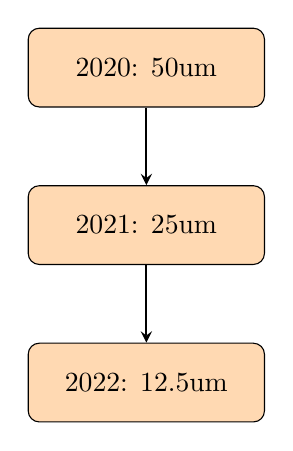
\begin{tikzpicture}[node distance=2cm]
\node (year1) [year] {2020: 50um};
\node (year2) [year, below of=year1] {2021: 25um};
\node (year3) [year, below of=year2] {2022: 12.5um};
\draw [arrow] (year1) -- (year2);
\draw [arrow] (year2) -- (year3);
\end{tikzpicture}
\end{center}
Note that our competitor, IBM, announced in May 2021 of its capability to manufacture entire transistors which are 2nm in width, which is 6250 times smaller than this projected feature size. Although their market is entirely different from ours, this fact makes it all the more reasonable that our technology should be able to reach a size 6250 times larger than the current leader in transistor sizes.

\subsection{Future Device Performance}
Since the projected minimum feature size is exactly half of current generation, the old area, power, and speed calculations can be appropriately multiplied to find the new dimensions.
\subsubsection{Inverter Dimensions}
The channel sizes decrease to 12.5um by 12.5um for nMOS, and 12.5um by 25um for pMOS. Additionally, the projected length of the whole inverter is halved from 200um to 100um. The width is also halved, from 75um to 37.5um. 
\\
\\This provides for a total area per nMOS channel of:
\\
\\\centerline{\emph{156.25 microns squared}}
\\
\\And a total area per pMOS channel of:
\\
\\\centerline{\emph{312.5 microns squared}}
\\
\\And a total area of the inverter of:
\\
\\\centerline{\emph{3750 microns squared}}

\subsubsection{Power}
\paragraph{Power Loss from Resistance} 
Given the formula for resistance used in power loss,
\\
\\\[R = \frac{L_{channel}}{W_{channel} \times H \times \mu \times N_D \times q} \]
\[R = \frac{\frac{1}{2} \times L_{channel}}{\frac{1}{2} \times W_{channel} \times H \times \mu \times N_D \times q} \]
\[R = 1 \times \frac{L_{channel}}{W_{channel} \times H \times \mu \times N_D \times q} \]
\\There is no change in resistive power loss. Thus, the calculations for resistive power do not change:
\[P_R = \frac{V_{DD}^2}{2R_P} \]
\[P_R = \frac{10V^2}{2 \times 891742465 \Omega} \]
\[P_R = 0.00000005607W \]
\[P_R \approx 56nW \]
\paragraph{Power Loss from Capacitance}
Given the formula for capacitance used in capacitive power loss,
\[C = \frac{W \times L \times \epsilon _{SiO2}}{H} \]
\[C = \frac{\frac{1}{2} \times W \times \frac{1}{2} \times L \times \epsilon _{SiO2}}{H} \]
\[C = \frac{1}{4} \times \frac{W \times L \times \epsilon _{SiO2}}{H} \]
The calculations for capacitive power change as follows:
\[P_C = f_{sw} \times \frac{1}{2} \times C_{out} \times V_{DD}^2 \]
\[P_C = \frac{1}{4} \times f_{sw} \times \frac{1}{2} \times C_{out} \times V_{DD}^2 \]
\[P_C = 0.000002248086W \]
\[P_C \approx 2304nW \]

\paragraph{Total Power Loss}
Thus, the total power loss changes to:
\[P \approx 2296nW \]

\subsubsection{Speed}
Given the formula for delay, the new delay can be calculated to be:
\[\tau _{HL} = \tau _{LH} = \frac{5 \times L_N^2}{\mu _N \times V_{DD}} \]
\[\tau _{HL} = \tau _{LH} = \frac{5 \times (\frac{1}{2} \times L_N)^2}{\mu _N \times V_{DD}} \]
\[\tau _{HL} = \tau _{LH} = \frac{1}{4} \times \frac{5 \times L_N^2}{\mu _N \times V_{DD}} \]
\[\tau _{HL} = \tau _{LH} = \frac{0.000000004464}{4}s\]
\[\tau _{HL} = \tau _{LH} = 0.000000001116s\]
\[\tau _{HL} = \tau _{LH} \approx 1.1ns\]


\\
\emph {\\This report represents my own work in accordance with R\&D Division regulations.}
\\
\includegraphics[width=5cm] {Daniel Simone signature}
\end{document} 